\documentclass[aspectratio=169]{../latex_main/tntbeamer}  % you can pass all options of the beamer class, e.g., 'handout' or 'aspectratio=43'
\usepackage{dsfont}
\usepackage{bm}
\usepackage[english]{babel}
\usepackage[T1]{fontenc}
%\usepackage[utf8]{inputenc}
\usepackage{graphicx}
\graphicspath{ {./figures/} }
\usepackage{algorithm}
\usepackage[ruled,vlined,algo2e,linesnumbered]{algorithm2e}
\usepackage{hyperref}
\usepackage{booktabs}
\usepackage{mathtools}

\usepackage{amsmath,amssymb}

\DeclareMathOperator*{\argmax}{arg\,max}
\DeclareMathOperator*{\argmin}{arg\,min}

\usepackage{amsbsy}
\newcommand{\vect}[1]{\bm{#1}}
%\newcommand{\vect}[1]{\boldsymbol{#1}}

\usepackage{pgfplots}
\pgfplotsset{compat=1.16}
\usepackage{tikz}
\usetikzlibrary{trees} 
\usetikzlibrary{shapes.geometric}
\usetikzlibrary{positioning,shapes,shadows,arrows,calc,mindmap}
\usetikzlibrary{positioning,fadings,through}
\usetikzlibrary{decorations.pathreplacing}
\usetikzlibrary{intersections}
\pgfdeclarelayer{background}
\pgfdeclarelayer{foreground}
\pgfsetlayers{background,main,foreground}
\tikzstyle{activity}=[rectangle, draw=black, rounded corners, text centered, text width=8em]
\tikzstyle{data}=[rectangle, draw=black, text centered, text width=8em]
\tikzstyle{myarrow}=[->, thick, draw=black]

% Define the layers to draw the diagram
\pgfdeclarelayer{background}
\pgfdeclarelayer{foreground}
\pgfsetlayers{background,main,foreground}

% Requires XeLaTeX or LuaLaTeX
%\usepackage{unicode-math}

\usepackage{fontspec}
%\setsansfont{Arial}
\setsansfont{RotisSansSerifStd}[ 
Path=../latex_main/fonts/,
Extension = .otf,
UprightFont = *-Regular,  % or *-Light
BoldFont = *-ExtraBold,  % or *-Bold
ItalicFont = *-Italic
]
\setmonofont{Cascadia Mono}[
Scale=0.8
]

\renewcommand{\ttdefault}{Cascadia Mono}

% scale factor adapted; mathrm font added (Benjamin Spitschan @TNT, 2021-06-01)
%\setmathfont[Scale=1.05]{Libertinus Math}
%\setmathrm[Scale=1.05]{Libertinus Math}

% other available math fonts are (not exhaustive)
% Latin Modern Math
% XITS Math
% Libertinus Math
% Asana Math
% Fira Math
% TeX Gyre Pagella Math
% TeX Gyre Bonum Math
% TeX Gyre Schola Math
% TeX Gyre Termes Math

% Literature References
\newcommand{\lit}[2]{\href{#2}{\footnotesize\color{black!60}[#1]}}

%%% Beamer Customization
%----------------------------------------------------------------------
% (Don't) Show sections in frame header. Options: 'sections', 'sections light', empty
\setbeamertemplate{headline}{empty}

% Add header logo for normal frames
\setheaderimage{
	% 
\includegraphics[height=\logoheight]{figures/TNT_darkv4.pdf}
	
\includegraphics[height=\logoheight]{../latex_main/figures/Leibniz-AI-Academy_Logo}
	% 
\includegraphics[height=\logoheight]{figures/logo_tntluh.pdf}
}

% Header logo for title page
\settitleheaderimage{
	% 
\includegraphics[height=\logoheight]{figures/TNT_darkv4.pdf}
	
\includegraphics[height=\logoheight]{../latex_main/figures/Leibniz-AI-Academy_Logo}
	% 
\includegraphics[height=\logoheight]{figures/logo_tntluh.pdf}
}

% Title page: tntdefault 
\setbeamertemplate{title page}[tntdefault]  % or luhstyle
% Add optional title image here
%\addtitlepageimagedefault{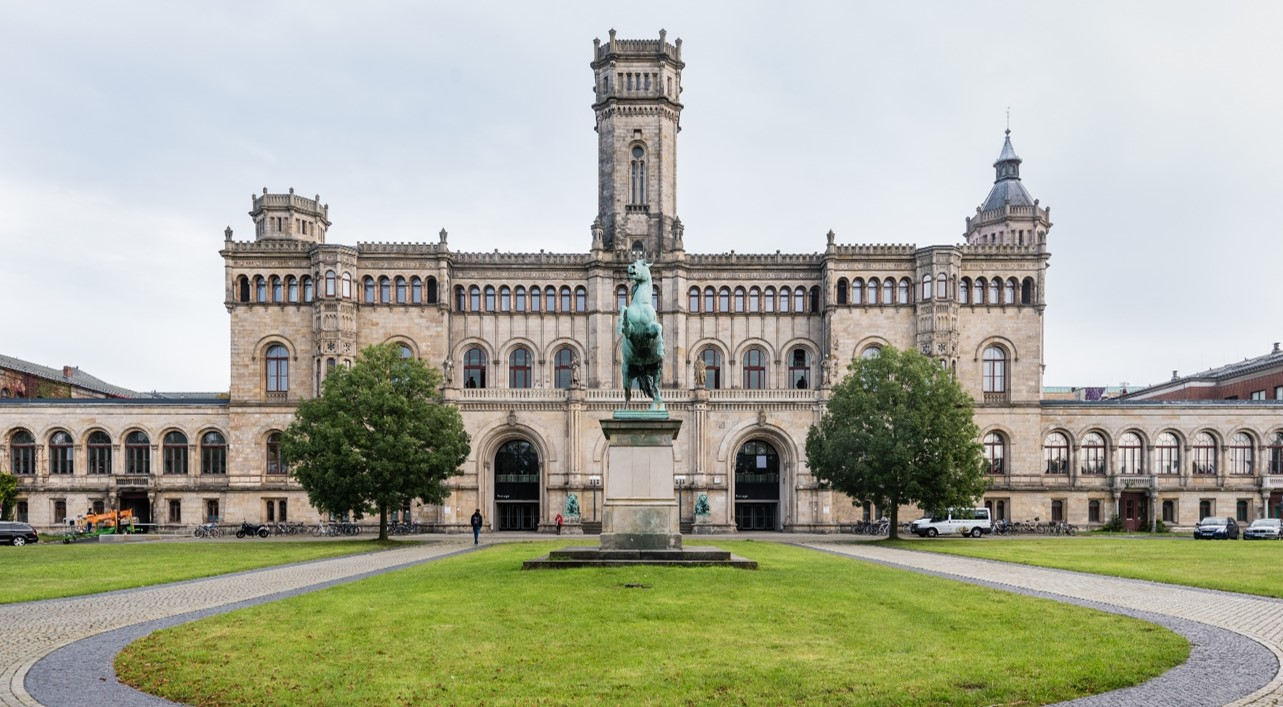
\includegraphics[width=0.65\textwidth]{figures/luh_default_presentation_title_image.jpg}}

% Title page: luhstyle
% \setbeamertemplate{title page}[luhstyle]
% % Add optional title image here
% \addtitlepageimage{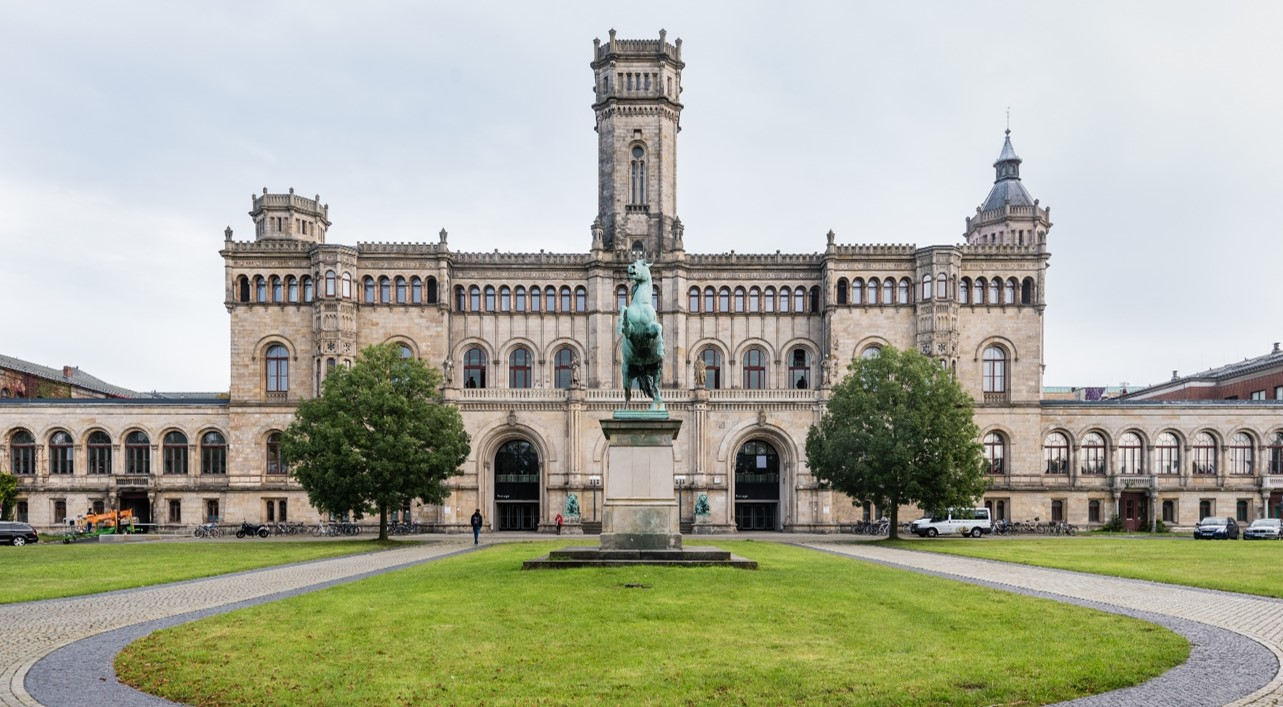
\includegraphics[width=0.75\textwidth]{figures/luh_default_presentation_title_image.jpg}}

\author[Abedjan \& Lindauer]{Ziawasch Abedjan \& \underline{Marius Lindauer}\\[1em]
	%
\includegraphics[height=\logoheight]{../latex_main/figures/luh_logo_rgb_0_80_155.pdf}\qquad
	
\includegraphics[height=\logoheight]{../latex_main/figures/DBIS_Kurzlogo.png}\qquad
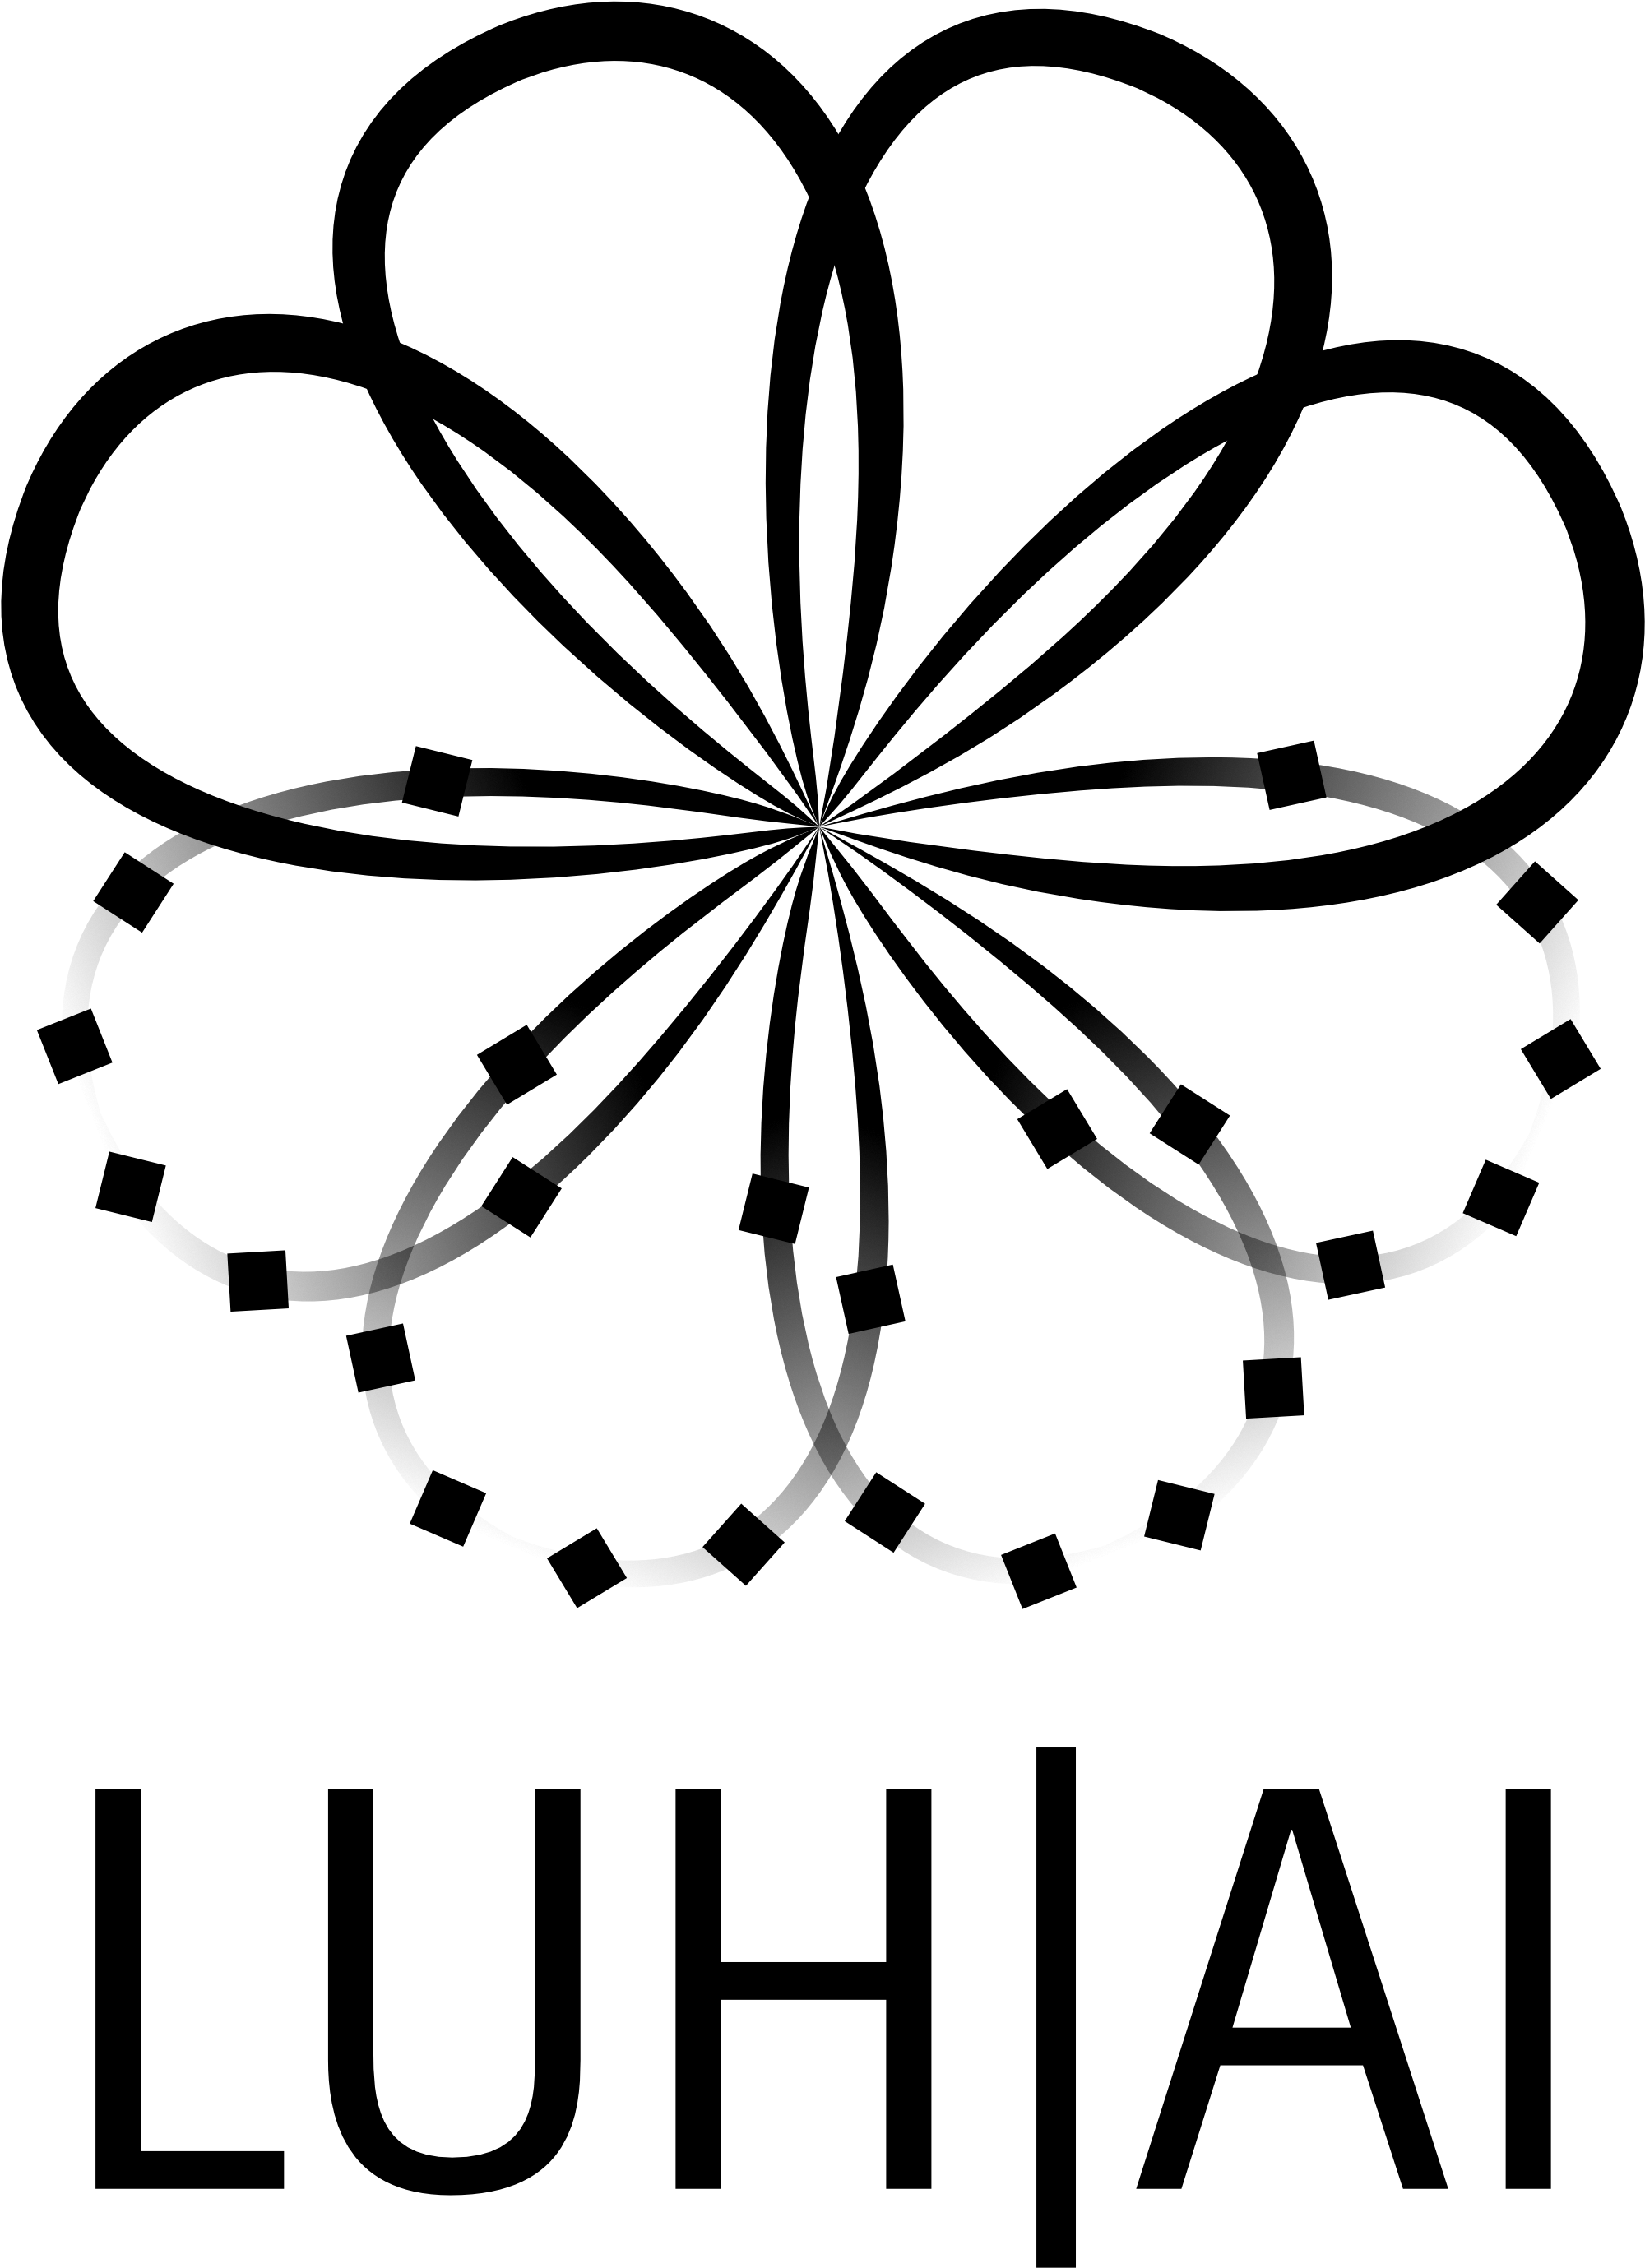
\includegraphics[height=\logoheight]{../latex_main/figures/logo_short_highres_black}\qquad

\includegraphics[height=\logoheight]{../latex_main/figures/Leibniz-AI-Academy_Logo}\qquad
%
\includegraphics[height=\logoheight]{../latex_main/figures/L3S.jpg}	
}
\date{\hspace{0.5em} {
\includegraphics[height=1.5em]{../latex_main/figures/Cc-by-nc-sa_icon.svg.png}}; extension of \href{https://ds100.org/fa21/}{[DS100]}
}


%%% Custom Packages
%----------------------------------------------------------------------
% Create dummy content
\usepackage{blindtext}

% Adds a frame with the current page layout. Just call \layout inside of a frame.
\usepackage{layout}


%%% Macros
%\renewcommand{\vec}[1]{\mathbf{#1}}
% \usepackage{bm}
%\let\vecb\bm

\title[Probability Samples]{DS: Data Sampling and Probability}
\subtitle{Probability Samples}

\graphicspath{ {./figure/} }
%\institute{}


\begin{document}
	
	\maketitle
		\begin{frame}{Probability sampling}
	    \begin{columns}
	        \begin{column}{.4\textwidth}
	            Why? One reason is to reduce bias, but that’s not the main reason!
	            \begin{itemize}
	                \item Random samples \textbf{can} produce biased estimates of population characteristics.
	                \begin{itemize}
	                    \item For example, if we’re estimating the maximum of a population.
	                \end{itemize}
	                \item But with random samples we are able to \textbf{estimate the bias and chance error}.
	                \begin{itemize}
	                    \item We can \textbf{quantify the uncertainty}.
	                \end{itemize}
	            \end{itemize}
	        \end{column}
	        
	        \begin{column}{.5\textwidth}
	            For our purposes, \textbf{probability samples} and random samples will mean the same thing.
             
	            \bigskip
	            A probability sample is a \textbf{type of sampling technique}.
	        \end{column}
	        
	    \end{columns}
	    
	\end{frame}
	
	
		\begin{frame}{Probability sampling}
	    \begin{columns}
	        \begin{column}{.4\textwidth}
	            In order for a sample to be a probability sample:
	            \begin{itemize}
	                \item You must be able to provide the chance that any specified set of individuals will be in the sample.
	               \item All individuals in the population do not need to have the same chance of being selected.
	                \item You will still be able to measure the errors, because you know all the probabilities.
	            \end{itemize}
	        \end{column}
	        
	        \begin{column}{.5\textwidth}
	            Not all probability samples are necessarily good.
	            \bigskip
             
	            For instance, suppose I have three students: Mustafa, Anna and Xia, and I want to sample two of them.
	            \begin{itemize}
	                \item I choose Mustafa with probability 1.
	                \item I choose either  Anna or Xia, each with probability $\frac{1}{2}$.
	            \end{itemize}
	            This is a probability sample (but it’s not great).

	        \end{column}
	        
	    \end{columns}
	    
	\end{frame}
	
	
		\begin{frame}{Some random sampling schemes}
	    \begin{columns}
	        \begin{column}{.7\textwidth}
	            A \alert{random sample with replacement} is a sample drawn \textbf{uniformly} at random \textbf{with replacement}.

	            \begin{itemize}
	                \item Random doesn’t always mean “uniformly at random,” but in this specific context, it does.
	            \end{itemize}
	            A \alert{simple random sample} is a sample drawn \textbf{uniformly} at random \textbf{without replacement}.
                 \begin{itemize}
	                \item Every individual has the same chance of being selected.
	                \item Every pair has the same chance as every other pair.
	                \item Every triple has the same chance as every other triple.
	                \item And so on.

	            \end{itemize}
	        \end{column}
	        
	        \begin{column}{.3\textwidth}
	            \begin{figure}
	                \centering
	                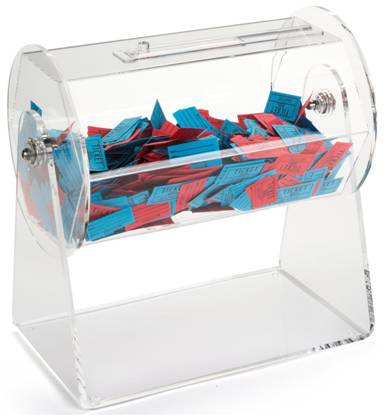
\includegraphics[scale=.5]{Bild14}
	            \end{figure}

	        \end{column}
	        
	    \end{columns}
	    
	\end{frame}
	
	
	
		\begin{frame}{Example Scenario}
	    \begin{columns}
	        \begin{column}{.3\textwidth}
	            Consider the following sampling scheme:

	            \begin{itemize}
	                \item Suppose a class roster has 1200 students listed alphabetically.
	                \item Pick one of the first 10 students on the list at random.
	                \item To create your sample, take that student and every 10th student listed after that (e.g. Students 8, 18, 28, etc).
	            \end{itemize}
	            Pause here and answer these questions!
                 
	        \end{column}
	        
	        \begin{column}{.6\textwidth}
	           Is this a probability sample?\\
	           \bigskip
	           Does each student have the same probability of being selected?\\
	           \bigskip
	           Is this a simple random sample?


	        \end{column}
	        
	    \end{columns}
	    
	\end{frame}
	
		\begin{frame}{Example Scenario (cont'd)}
	    \begin{columns}
	        \begin{column}{.3\textwidth}
	            Consider the following sampling scheme:

	            \begin{itemize}
	                \item Suppose a class roster has 1200 students listed alphabetically.
	                \item Pick one of the first 10 students on the list at random.
	                \item To create your sample, take that student and every 10th student listed after that (e.g. Students 8, 18, 28, etc).
	            \end{itemize}
                 
	        \end{column}
	        
	        \begin{column}{.6\textwidth}
	           Is this a probability sample?
	           \begin{itemize}
	               \item Yes. If my sample is [n, n + 10, n + 20, …, n + 1190], where $0 \leq n \leq 10$, the probability of that sample is $\frac{1}{10}$
	               \item Otherwise, the probability is 0.
	               \item Only 10 possible samples!
	           \end{itemize}
            \pause
	           Does each student have the same probability of being selected?
	           \begin{itemize}
	               \item Yes. Each student is chosen with probability $\frac{1}{10}$. 
	           \end{itemize}
                \pause
	           Is this a simple random sample?
                \begin{itemize}
                    \item No. The chance of selecting (8, 18) is 1/10; the chance of selecting (8, 9) is 0.
                \end{itemize}

	        \end{column}
	        
	    \end{columns}
	    
	\end{frame}
	
		
	
	\begin{frame}{A very common approximation}
	    \begin{itemize}
	        \item A common situation in data science:
	        \begin{itemize}
	            \item We have an enormous population.
	            \item We can only afford to sample a relatively small number of individuals.
	        \end{itemize}
	        \item If \textbf{the population is huge compared to the sample size}, then random sampling with and without replacement are pretty much the same.
	        \begin{itemize}
	            \item For instance, if our population size is in the thousands, and we’re sampling 100 people, removing those 100 doesn’t change the population very much.
	        \end{itemize}
	        \item Probabilities of sampling with replacement are much easier to compute!
	    \end{itemize}
	\end{frame}
	
\end{document}